\section{Behavior Results}
\label{sec:behave_result}
To answer RQ3, we investigate time-to-action and remaining credit differences across experiment conditions. Time-to-action is a widely used metric in decision sciences to understand individual behaviors. For example,~\textcite{payneAdaptiveDecisionMaker1993} theorized that longer decision time represents more complex and deeper cognitive processing. Additionally, resource allocation strongly influences decision making. \textcite{chengCanShowWhat2021} showed that the number of given credits influences the validity of QV. Decision science studies like \textcite{Shah2015a} and \cite{debruijnPovertyEconomicDecision2022} showed how scarcity influences decisions, increases risk aversion, and adds cognitive load. In this section, we use these two measures as proxies to understand participant behaviors. We publicly shared all analyzed participant interaction data\footnote{link-to-github} to support transparency and facilitate further research.

\newsavebox{\savefig}

\begin{figure}[htbp]
    \centering
    \savebox{\savefig}{
        \begin{minipage}{0.78\pdfpageheight}
            \begin{subfigure}[b]{0.26\pdfpageheight}
                \centering
                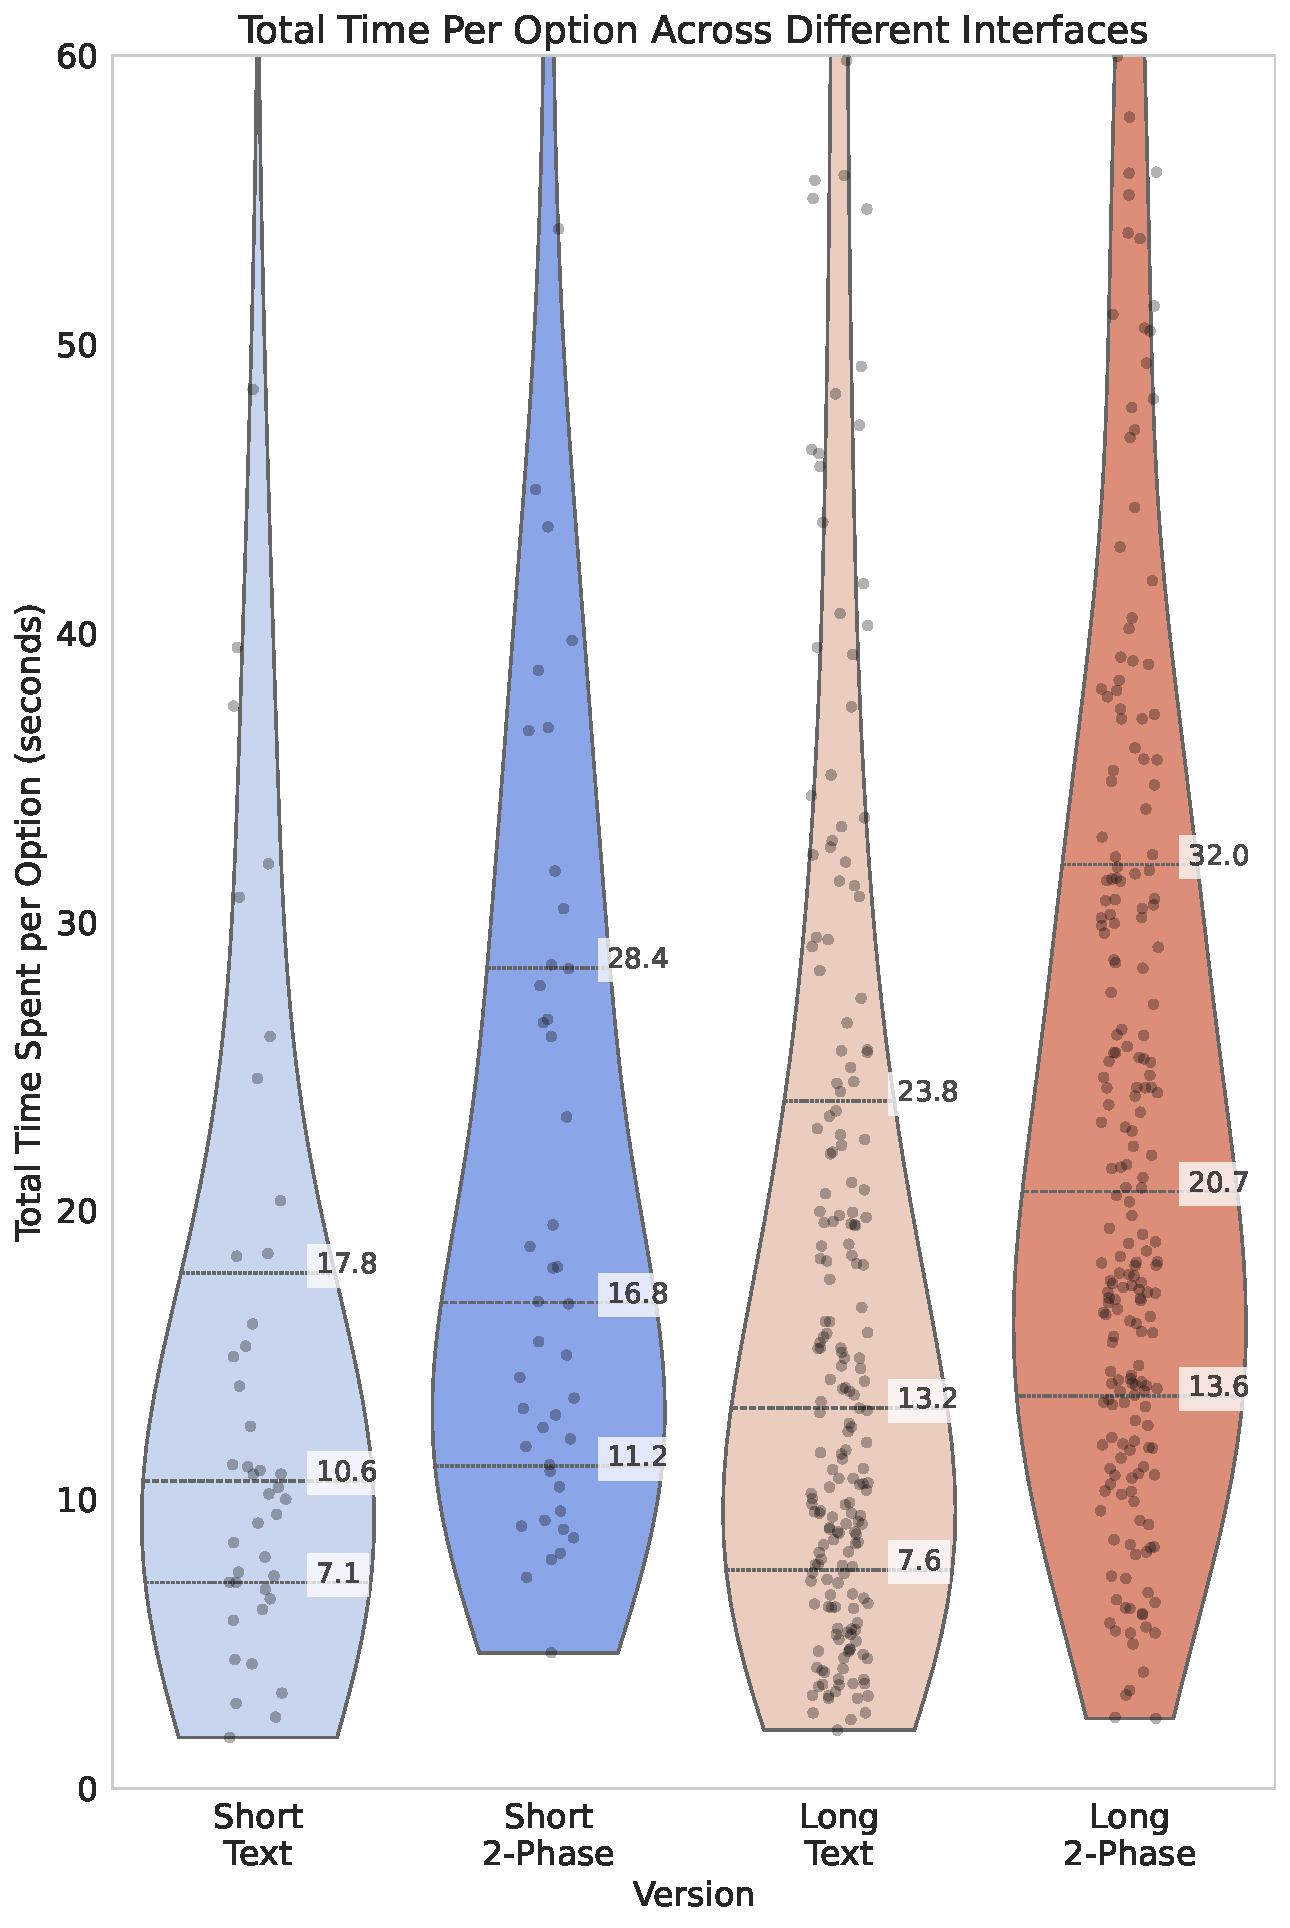
\includegraphics[width=\textwidth]{content/image/results/total_time_per_option.pdf}
                \caption{Total Time per option}
                \label{fig:total_time}
            \end{subfigure}
            % \hfill
            \begin{subfigure}[b]{0.26\pdfpageheight}
                \centering
                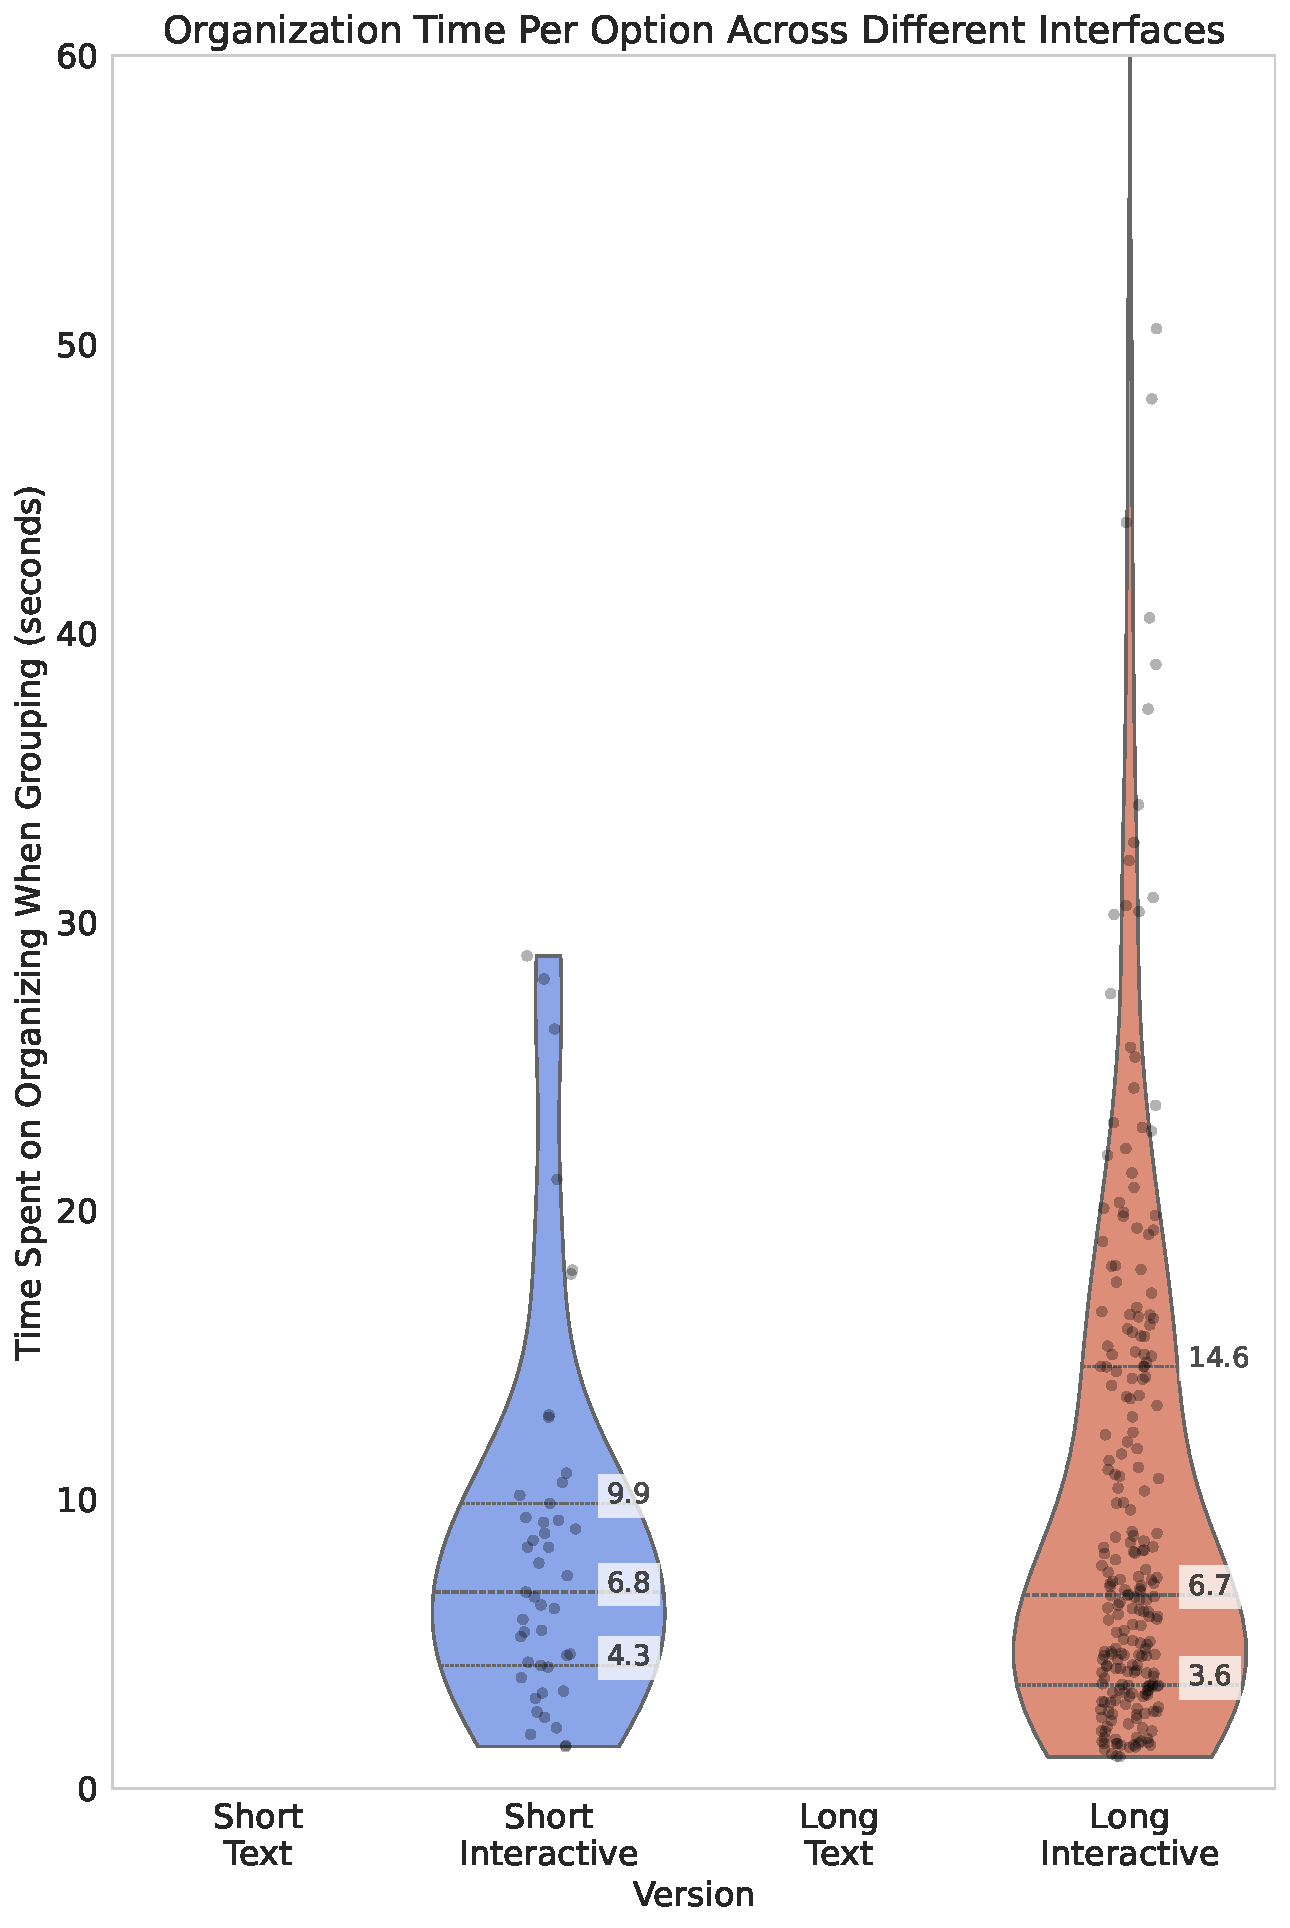
\includegraphics[width=\textwidth]{content/image/results/org_time_per_option.pdf}
                \caption{Organization Time per option}
                \label{fig:org_time}
            \end{subfigure}
            % \hfill
            \begin{subfigure}[b]{0.26\pdfpageheight}
                \centering
                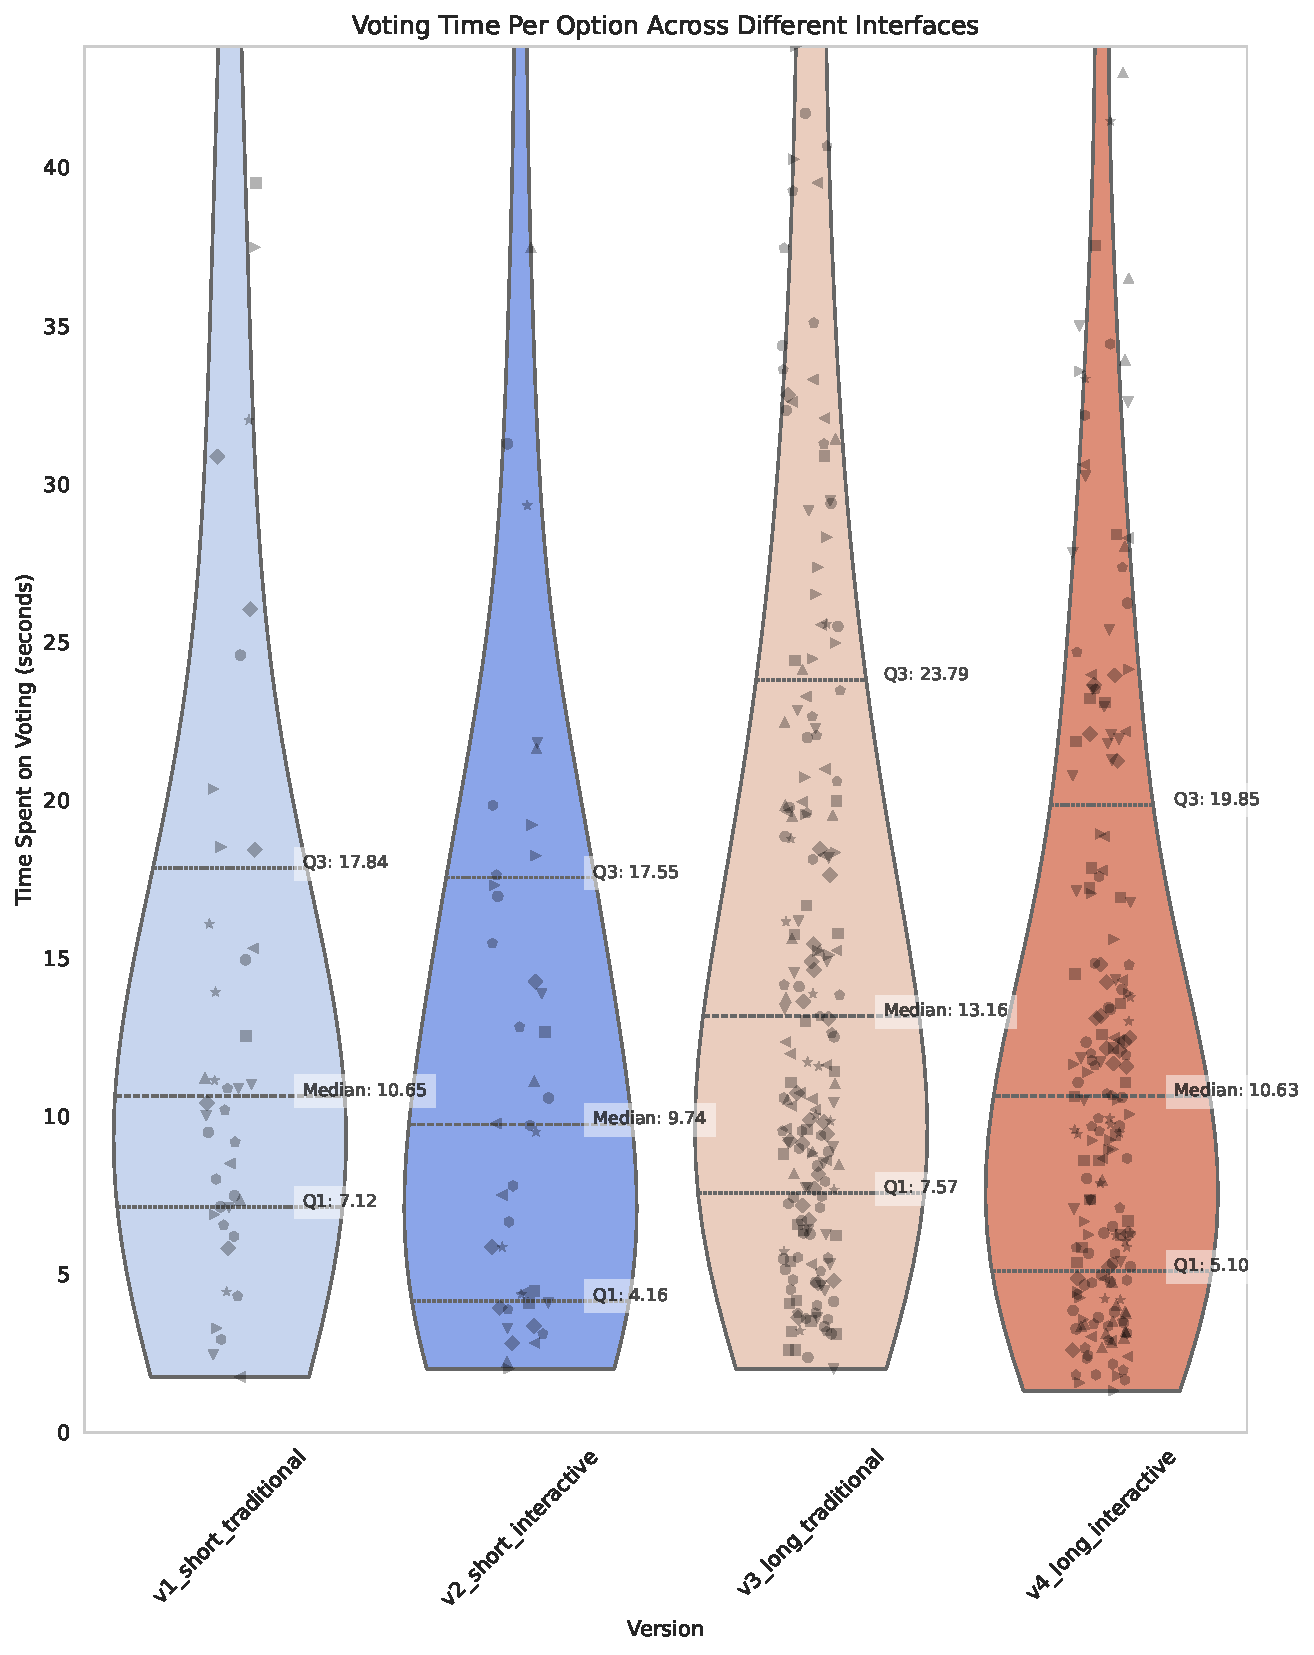
\includegraphics[width=\textwidth]{content/image/results/voting_time_per_option.pdf}
                \caption{Voting Time per option}
                \label{fig:vote_time}
            \end{subfigure}
        \end{minipage}
    }
    \rotatebox{90}{%
        \begin{minipage}{\wd\savefig}
            \usebox{\savefig}
            \caption{Swimlane Diagram}
        \end{minipage}
    }
    \label{fig:time_per_option_full}
\end{figure}


\subsection{Time Spent per Options}
\label{sec:time_per_option}
Our first analysis focuses on understanding how much time participants spent per option across different stages and experiment conditions. Based on the QS system log, we can derive the following detailed logs of participant actions:~\textit{the option}  involved in the interaction,~\textit{the type of interaction} (such as updating a certain number of votes), and~\textit{the time} between this interaction and the previous one.

We aggregate all the time spent on each option as the total time spent for that option. Organization time includes the time participants spent placing options into preference categories and the drag-and-drop time associated with each option during the organization phase. Voting time strictly refers to the time participants took to update vote values for each option. To minimize noise, we intentionally drop all the time participants spent on the first option in the organization phase or voting phase. The goal is to exclude time spent on reading the prompt, forming their preference, or understanding the interface.

Figure~\ref{fig:time_per_option_full} each dot represents one option for one participant. Figure~\ref{fig:total_time} shows total time, figure~\ref{fig:org_time} shows organization time, and figure~\ref{fig:vote_time} shows voting time. The violin plot shows the distribution of the dots and the three horizontal lines represent the median, 25th percentile, and 75th percentile of the time spent for that interface. We limited the y-axis to 1 minute to improve visualization clarity.

Participants spent more time on the interactive interface than the text interface in both short and long surveys. A non-parametric Mann-Whitney U test confirmed this observation. For the long QS, the Mann-Whitney U test results showed a significant difference between the text interface and the interactive interface ($U=15536$, $p<0.0000001$). The effect size was small (Rank-biserial: $-0.304$, Cohen's d: $-0.030$) and the power of the test was $0.061$. For the short QS, the Mann-Whitney U test results showed a significant difference between the text interface and the interactive interface ($U=573$, $p=0.01$). The effect size was small (Rank-biserial: $-0.37$, Cohen's d: $-0.082$) and the power of the test was $0.066$. These results indicate that participants spent slightly less time on the text interface. This is expected as organizing options in the interactive interface takes more time. We break down the total time spent into organization time and voting time in Figure~\ref{fig:org_time} and Figure~\ref{fig:vote_time}.

We observed minimal difference in organization time (Figure~\ref{fig:org_time}) between short and long interface. The interface was designed with this in mind given that options are shown one at a time, and participants can drag and drop them into the preference categories when needed. Examining the voting time (Figure~\ref{fig:vote_time}), there is no significant difference in voting time between the text and interactive interfaces in the short survey ($p>0.4$, Power=$0.051$). However, in the long QS, there is a statistically significant difference ($U=24053$, $p<0.005$) in voting time between the text and interactive interfaces. The effect size was small (Rank-biserial: $0.167$, Cohen's d: $0.017$) and the power of the test was $0.053$. This indicates that participants spent slightly less time on the interactive interface in the long survey. This supports our hypothesis that the two-step design in the interactive interface facilitates more efficient decision-making, especially in longer surveys.

\subsection{Budget and Voting Behaviors}
To further analyze participant behaviors, we break down the aggregated time from the previous analysis and examine fine-grain interactions. Specifically, we examine if there are differences among behavior across interfaces. As we outlined, credit scarcity might influence decision making.  Figure~\ref{fig:voting_all} plots the time of voting actions over the remainder of the participant's budget across the text and interactive interface across all four groups. Each bar shows the number of actions accumulated across participants at specific percentages of remaining credits. A KDE plot is provided to better visualize the trends. We chose not to follow ~\textcite{quarfoot2017quadratic} focusing on the number of accumulated votes over an individual's time given that each individual's total time spent differ across experiment conditions.

Comparing experiment groups, we see fewer differences in the short QS but different interaction distributions between the two interfaces in the long QS. Given the significant differences in voting time between the text and interactive interfaces for the long QS, we focus on deciphering the voting action changes between these two conditions in this subsection.

\begin{figure}[ht]
    \centering
    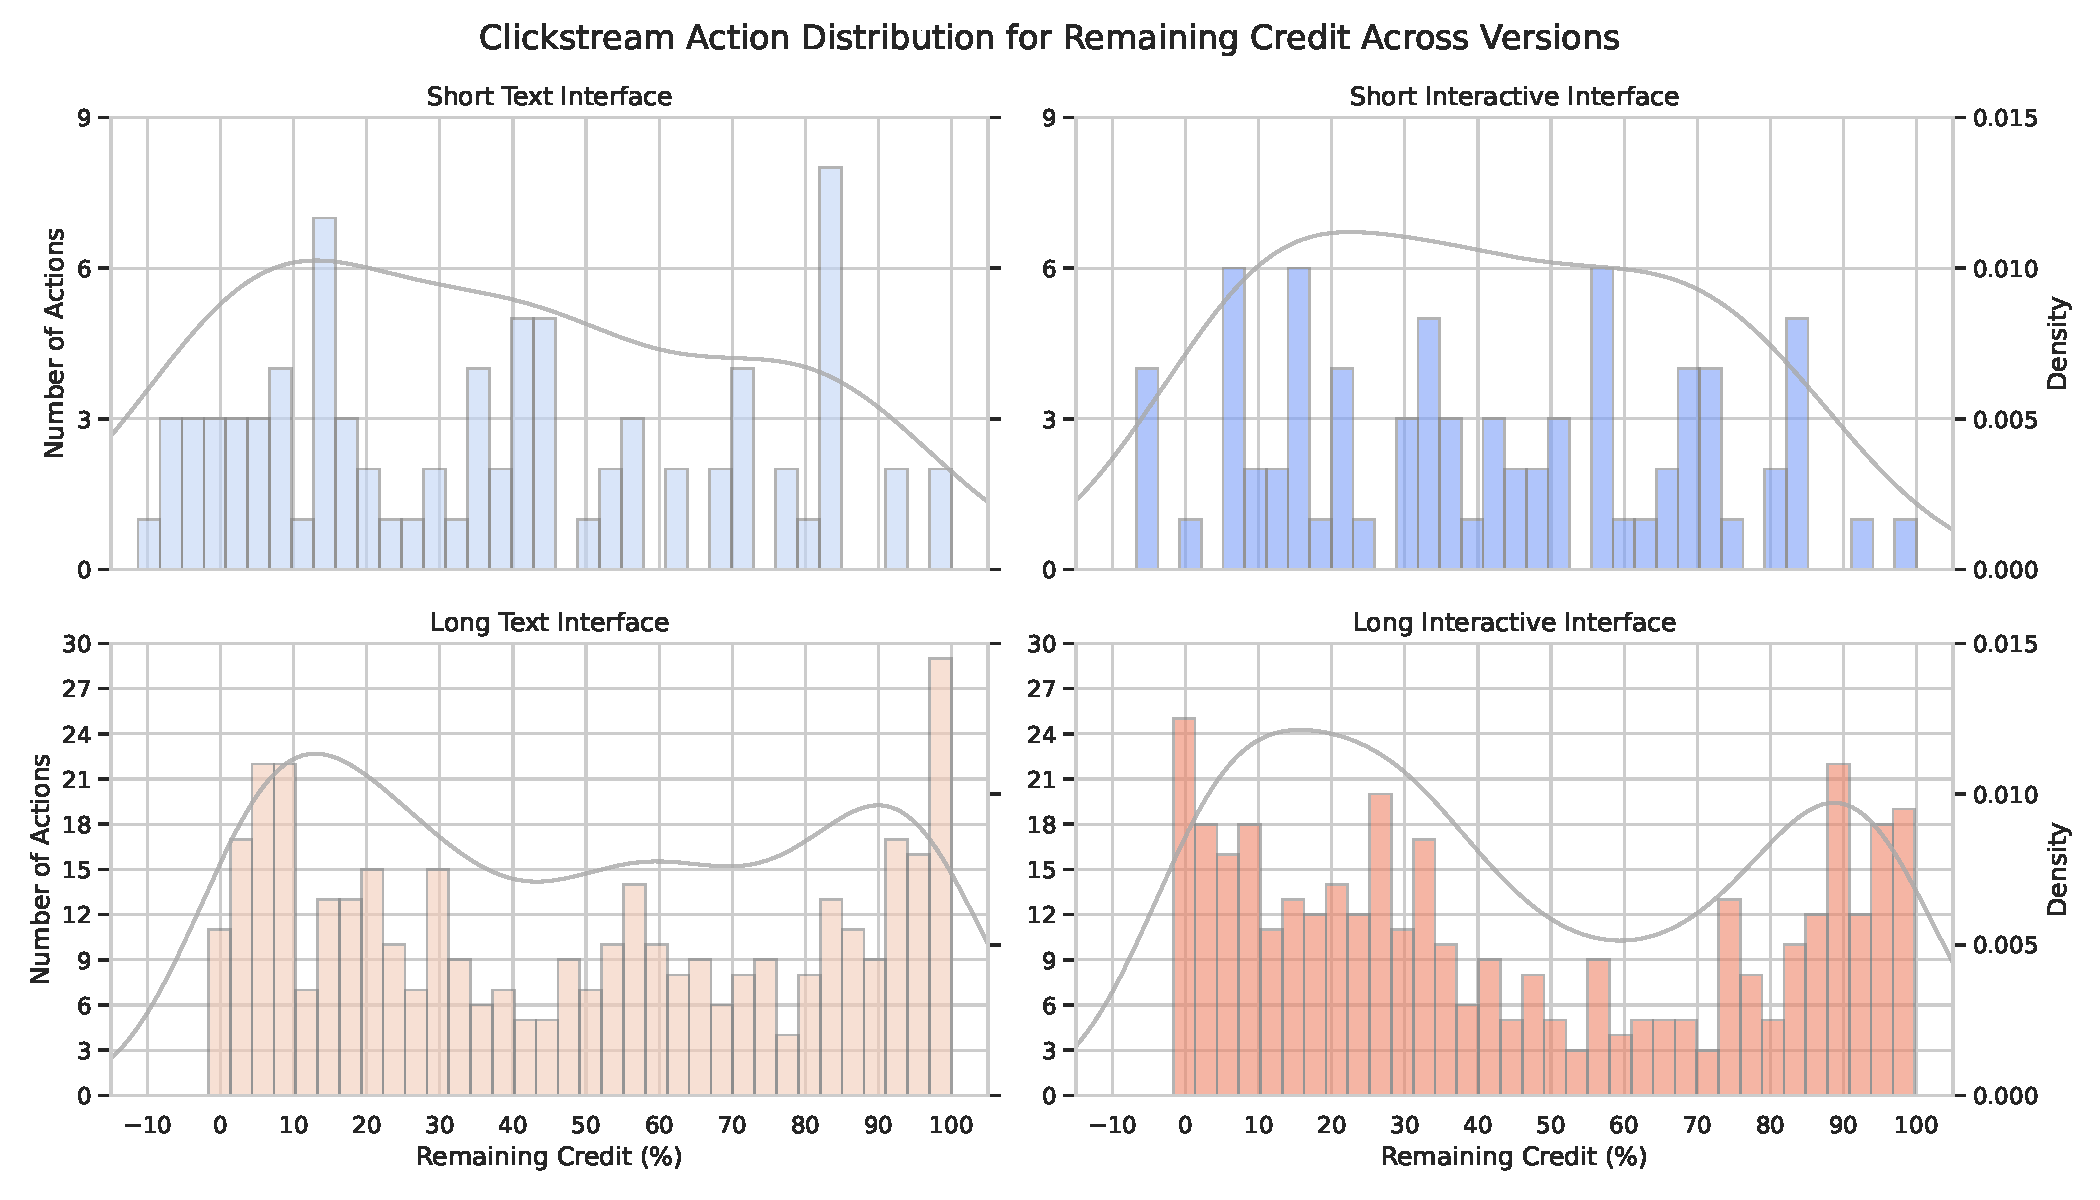
\includegraphics[width=\textwidth]{content/image/results/clickstream_action_distribution.pdf}
    \caption{Voting actions across all options (needs to update chart text, remove normalization, and change the dot colors.)}
    \label{fig:voting_all}
\end{figure}

In Figure~\ref{fig:voting_all}, we see two distinct patterns between the short survey and the long survey in terms of participant behaviors. In long surveys, participants exhibited more actions both when the budget was abundant and when it began to run out. This pattern was more pronounced with the long interactive interface. We further separated the behaviors where participants made large or small changes to the options, specifically for the long version. In Figure~\ref{fig:voting_v3_v4}, we define an adjustment of four or more votes as large, which we plotted in the first row of the figure. Adjustments of two or fewer votes are considered small, which is $10\%$ of the possible values one can choose among the maximum of 21 votes.

\begin{figure}[ht]
    \centering
    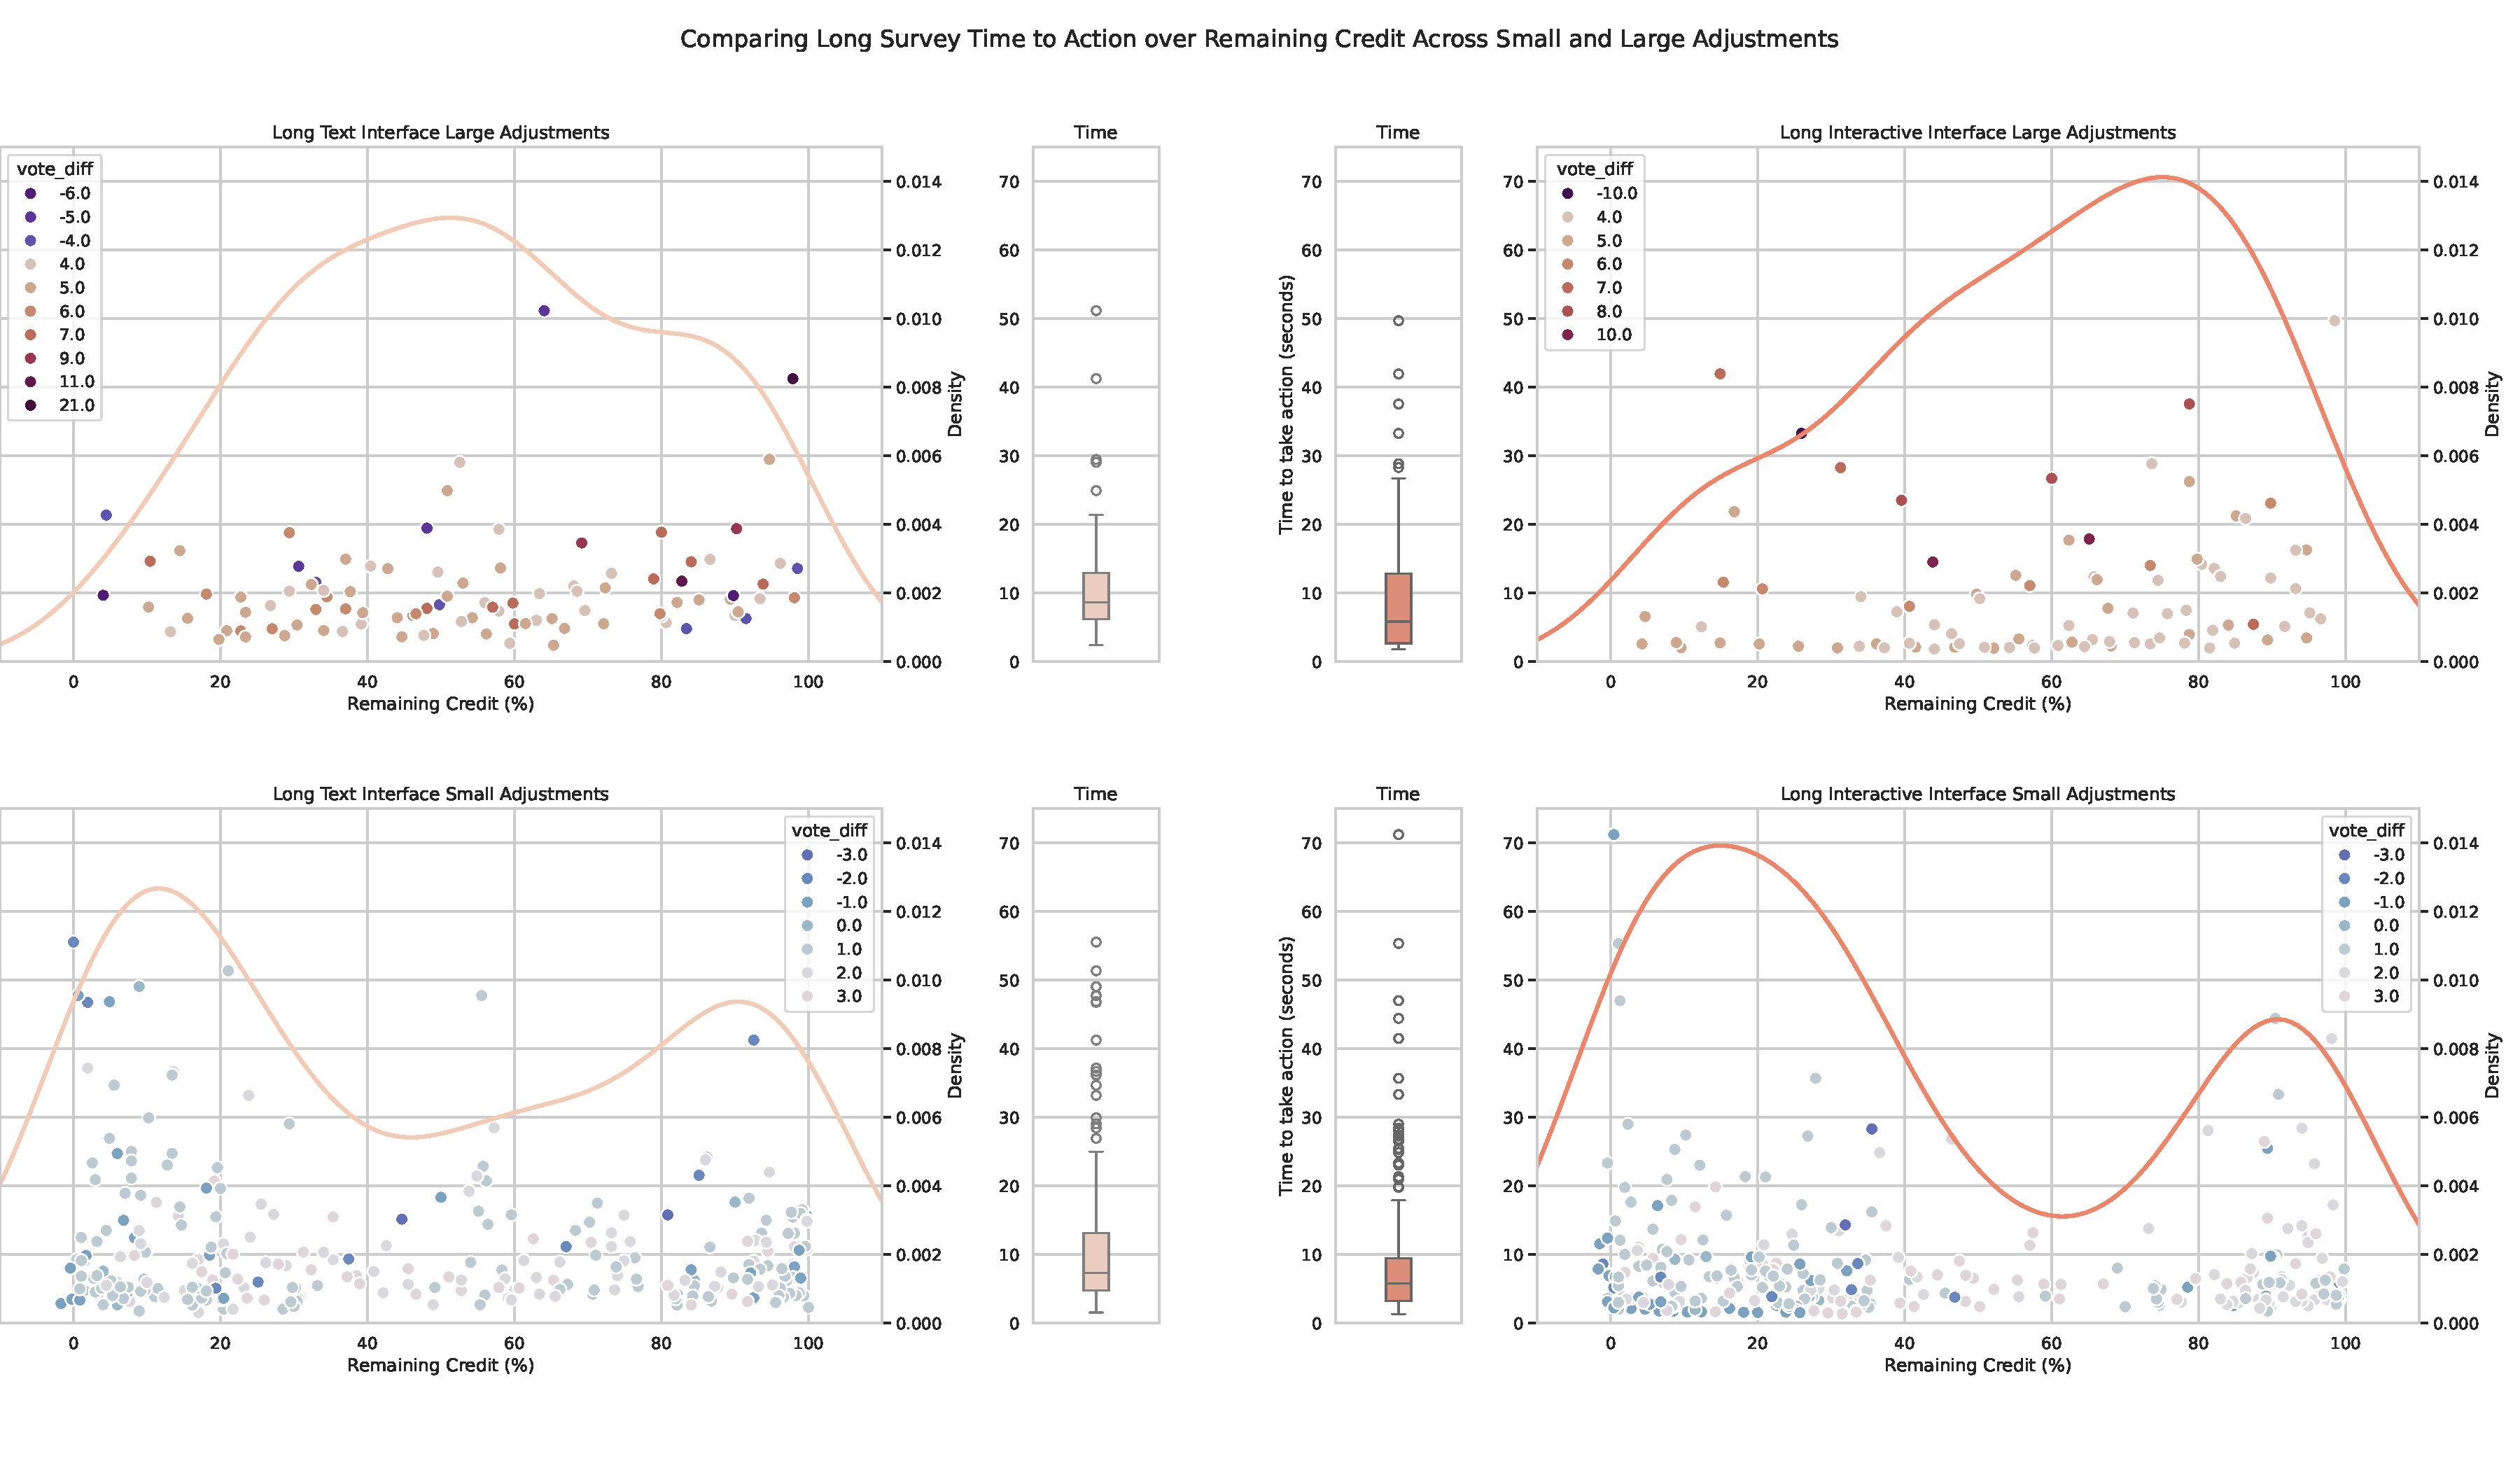
\includegraphics[width=\textwidth]{content/image/results/combined_density_plots.pdf}
    \caption{Breakdown of voting actions (needs to update chart text)}
    \label{fig:voting_v3_v4}
\end{figure}

Instead of showing the number of actions, we plotted all actions against the time it took to make them. Revisiting the KDE curve in the second row in Figure~\ref{fig:voting_all} and the curve of the second row in Figure~\ref{fig:voting_v3_v4} which represents the small vote adjustment across both interfaces, we see a stronger bimodal action distribution. In fact, the bimodal distribution is more pronounced in the interactive interface. This suggests that participants make small adjustments both at the beginning and towards the end of the QS. However, the interactive interface shows more frequent and faster edits towards the end. Visually, dots are more clustered in the long interactive interface for small vote adjustments compared to the long text interface. The Mann-Whitney U Test on the time spent on small vote adjustments showed significant differences ($U=13037$, $p<0.001$), with a small effect size (Rank-biserial: $0.227$, Cohen's d: $0.195$) and a power of $0.381$. Based on the KDE plots in the first row of Figure~\ref{fig:voting_v3_v4}, participants also made more large vote adjustments early on that spread more equally compared to the text interface. This indicates that participants had a clearer idea of how to distribute their credits across the options.

In interviews, five participants highlighted the importance of the interface's flexibility and their use of an incremental, iterative approach. All these participants used the interactive interface. While this doesn't mean participants using the text interface didn't take an iterative approach, it highlights that the interactive interface encouraged iterative and incremental updates. As one participant pointed out:

\begin{displayquote}
I like the fact that it remembers everything that you know. If if you make a mistake, that you don't lose all the work that you've already done. so I think that's very important is that it's an iterative process.

\noindent \hfill -- S019, long interactive interface.
\end{displayquote}

~\textbf{In summary, the interactive interface allowed participants to better structure their preferences and make faster iterative adjustments, as designed based on the differentiation and consolidation theory.} In other words, we show~\textit{different} voting behaviors presented across long text and interactive interface, hence~\textbf{rejecting} the alternative plausible explaination on the hightened cognitive load in the long interactive interface due to a pure increase of cognitive load Due to interactivity, hence further concluding that the interactive interface prevents satisficing from cognitive overload in long QS.

% This suggests that participants in the interactive interface are more likely to make larger adjustments to their votes. This is consistent with the observation that participants in the interactive interface spent more time on voting actions in the long survey. We also see a cluster of voting actions in the bottom left corner of the interactive interface for small vote adjustments. This suggests that participants in the interactive interface are more likely to make small adjustments when their budget is running low. This is consistent with the observation that participants in the interactive interface spent less time on voting actions in the long survey.
% First, surface the bimodal action distribution in both plots, with a even stronger signal for long interactive interface participants. Second, the plot demonstrated a clear cluster of voting actions in the bottom left corner of the interactive interface for small vote adjustments. In other words, participants made much smaller but more rapid adjustments when their budgets were running low. Second, larger adjustments are made when the participants have more options comparing the two plots on the first row. We interpret this behavior as participants in the interactive interface have constructed a clearer image of option preferences and, hence, have the ability to take larger strides in allotting their budget and deciding the number of votes at the beginning of the survey. Toward the end, participants using the interactive interface are then making fine-tuned adjustments to ensure that their preferences are reflected in their submissions.

% add qualitative support


% Ti-Chung Cheng: So what elements of the software interface do you dislike, or like the most, if any, when expressing your preferences on responding to societal issues?
% S009: Hmm! What I like the most actually, probably the sorting function. I think that it really helped me organize my thoughts really, clearly, in terms of what I would dislike the most. really, not that much. I would say. yeah, also, like how we could categorize it, like even within the voting stage rather than just at the categorization stage. 

% Ti-Chung Cheng: Can you tell me a little bit more about the screen? How did the vertical screen help you?
% S037: I think because it helps the layout of, because it's like a long 3 bar. So it's easier for you to to drag and drop, and you can actually sort it, judging by the votes. But I do not do that. But I think this layout is could be helpful in that aspect.


